\documentclass[tikz,border=10pt]{standalone}
\usetikzlibrary{angles}
\begin{document}
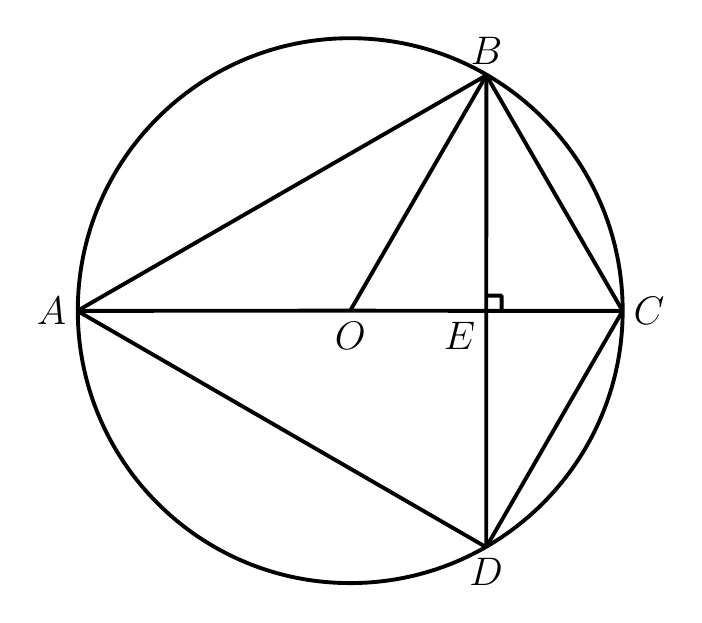
\begin{tikzpicture}[line width=1.4pt, line join=round]
\coordinate (A) at (-3.485,0.013);
\coordinate (B) at (1.710,3.005);
\coordinate (C) at (3.440,0.013);
\coordinate (D) at (1.708,-2.988);
\coordinate (O) at (-0.019,0.016);




\coordinate (E) at (1.709,0.013);


\draw (O) circle[radius=3.460];


\draw (A) -- (O);
\draw (O) -- (E) -- (C);


\draw (B) -- (E) -- (D);


\draw (A) -- (B);
\draw (A) -- (D);
\draw (B) -- (C);
\draw (D) -- (C);
\draw (B) -- (O);


\draw pic[draw, angle radius=0.194cm] {right angle=C--E--B};


\node[left]        at (A) {\fontsize{14.5}{17.4}\selectfont $A$};
\node[right]       at (C) {\fontsize{14.5}{17.4}\selectfont $C$};
\node[above]       at (B) {\fontsize{14.5}{17.4}\selectfont $B$};
\node[below]       at (D) {\fontsize{14.5}{17.4}\selectfont $D$};
\node[below]       at (O) {\fontsize{14.5}{17.4}\selectfont $O$};
\node[below left]  at (E) {\fontsize{14.5}{17.4}\selectfont $E$};
\end{tikzpicture}
\end{document}